\documentclass[12pt, a4paper]{article}
\title{Интерференция лазерного излучения (4.5.2)}
\author{Стеценко Георгий, Б02-312}
\date{}
% !TeX encoding = UTF-8

\usepackage{geometry}
\usepackage{amsmath, amsfonts, amssymb, amsthm} % стандартный набор AMS-пакетов для математ. текстов
\usepackage{mathtext}
\usepackage[utf8]{inputenc} % кодировка utf8
\usepackage[russian]{babel} % русский язык
\usepackage[pdftex,dvipsnames]{xcolor} % работа с цветами
\usepackage[pdftex]{graphicx} % графика (картинки)
\usepackage{tikz,pgfplots} % рисунки
\usepackage{indentfirst}
%\usepackage[labelfont=bf,labelsep=endash,skip=3pt]{caption} % подпись картинок
% \usepackage{fancyhdr,pageslts} % настройка колонтитулов
\usepackage{enumitem} % работа со списками
\usepackage{floatrow,multicol,multirow,longtable,hhline} % работа с таблицами
\usepackage{float,wrapfig} % плавающие объекты
\usepackage{tcolorbox} % рамка вокруг текста
%\usepackage[calc]{datetime2} % дата
\usepackage{bm} % жирное начертание в формулах
\usepackage{physics} % физический пакет
\DeclareMathAlphabet\mathbfcal{OMS}{cmsy}{b}{n}
\usepackage{pgfornament} % красивые рюшечки и вензеля
\usepackage{mdframed}
\usepackage{derivative}
\usepackage{mathrsfs} %EDS
\usepackage{soul} % strikethorugh
%\usepackage{boondox-cal}

% ----------------------------------------
% Настройка шрифта

% Просто закооментируйте следующую строчку, если не работает. Будет другой шрифт, правда :(
% \usepackage{pscyr}

% ----------------------------------------
% Стилевые настройки

\usepackage{boldline} % жирная линия после таблиц (чтобы не было ошибок, этот пакет должен подключаться именно тут!)
\floatsetup[table]{style=Plaintop,floatrowsep=qquad} % настройка оформления таблиц
\setlist[enumerate,itemize]{leftmargin=5mm,itemindent=10mm,itemsep=0mm,
listparindent=0em,labelsep=2mm,topsep=2mm,labelwidth=4mm} % настройки списков

\setlength{\columnsep}{0.5cm} % расстояние между колонками
\setlength{\parskip}{1pt} % расстояние до текста от колонтитула

%\usepackage{titlesec} % управление оформлением section
%\renewcommand{\thesection}{\Roman{section}}
%\titleformat{\section}[block]{\bfseries\large}{\thesection.}{5pt}{}

% ----------------------------------------
% Настройки полей
\geometry{
  left=10mm,
  top=10mm,
  right=10mm,
  bottom=15mm,
  marginparsep=0mm,
  marginparwidth=0mm,
  headheight=0pt,
  headsep=0pt,
footskip=20pt}

% ----------------------------------------
% Настройки колонтитулов и нумерации страниц
\pagenumbering{arabic}



\newcounter{ntask}
\setcounter{ntask}{0}


\newcommand{\arsh}{\mathrm{arsh} \,\,}
\newcommand{\arch}{\mathrm{arch} \,\,}
\newcommand{\arth}{\mathrm{arth} \,\,}
\newcommand{\arcth}{\mathrm{arcth} \,\,}
\renewcommand{\Re}{\operatorname{Re} \,}
\newcommand{\EDS}{\mathscr{E}}
\newcommand{\diffract}[1]{\frac{\mathrm{d}#1}{\mathrm{d}t}}

\newcommand{\kHz}{~\mathrm{kHz}}
\newcommand{\GHz}{~\mathrm{GHZ}}
\newcommand{\us}{~\mathrm{\mu s}}
\newcommand{\J}{\mathcal{J}}
\newcommand{\uA}{~\mathrm{\mu A}}
\newcommand{\mim}{~\mathrm{mm}}
\newcommand{\V}{\mathcal{V}}
\addto\captionsrussian{\def\refname{Источники}}

\begin{document}
\maketitle

\section{Аннотация}
\sloppy \textbf{Цель работы}: Исследовать зависимость видности интерфереционной
картины от разности хода интерферирующих лучей и от их поляризации.

\textbf{Оборудование и материалы}: He-Ne лазер, интерферометр Майкельсона с
подвижным зеркалом, фотодиод с усилителем, осциллограф С1-76, поляроид,
линейка.

\section{Теоретические сведения}
Лазер представляет собой интерферометр Фабри-Перо -- газовую трубку с двумя
параллельными зеркалами по обе стороны. Пусть $\Delta F$ -- половина диапазона
генерации лазера, а $\Delta \nu$ -- межмодовое расстояние. Тогда межмодовое
расстояние выражается как
\begin{equation}
    \Delta \nu = \dfrac{c}{2L}
\end{equation}
При этом число мод можно оценить как
\begin{equation}
    N \approx 1 + \dfrac{2\Delta F}{\Delta \nu}.
    \label{eq:mode}
\end{equation}
\eqref{eq:mode}
\paragraph*{Видность}
Видность интерфереционной картины -- параметр, определяемый формулой
\begin{equation}
    \V = \dfrac{I_{max} - I_{min}}{I_{max} + I_{min}},
\end{equation}
где $I_{max}$, $I_{min}$ -- максимальная и минимальная интенсивности света интерфереционной картины вблизи выбранной точки. Разобьём его на произведение функций параметров установки
$$
    \V = \V_1 \V_2 \V_3.
$$

Здесь $\V_1$
\begin{equation}
    \V_1 = \dfrac{2\sqrt{\delta}}{1+\delta},
\end{equation}
где $\delta = \frac{B_m^2}{A_m^2}$, $A_m^2$ и $B_m^2$ -- интенсивности волн. Параметр $\delta$ выражает отношение интенсивностей интерферирующих волн.\\

Величина $\V_2$ зависит от геометрической разности хода интерферирующих волн,
$$ \V_2 = \dfrac{\sum\limits_n A^2_n \cos \frac{2\pi \Delta \nu n
            l}{c}}{\sum\limits_n A_n^2}, $$ где $l$ -- разность хода, $\Delta \nu$ --
спектральный состав излучения, $A_n^2$ -- интенсивности мод.
\begin{figure}[H]
    \begin{center}
        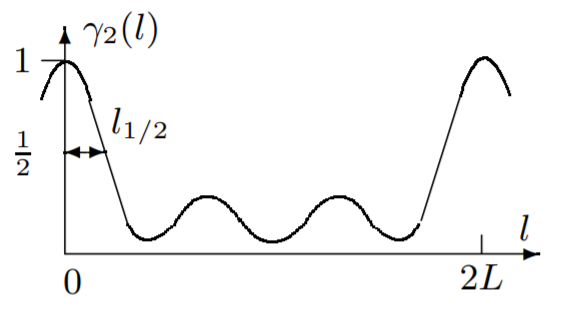
\includegraphics[scale=0.6]{pics/1.png}
    \end{center}
    \caption{Зависимость $\V_2(l)$.}
\end{figure}
\noindent Приблизим $\V_2$ вблизи максимума
$$
    \V_2 = e^{-\left(\frac{\pi \Delta F l}{c}\right)^2}
$$
Таким образом, ма имеем гауссову зависимость видности от разности хода $\V_2(l)$ с полушириной
\begin{equation}
    l_{1/2} = \dfrac{c}{\pi \Delta F}\sqrt{\ln 2} \approx \dfrac{0.26 c}{\Delta F}.
\end{equation}

Величина $\V_3$ соответсвует тому факту, что при интерференции поляризованных
волн интерфирируют лишь компоненты, поляризованные одинкаово. Необходимо
рассмотреть различные случаи поляризации лазера. Пусть на входе в ДК свет
поляризован по кругу. Тогда имеем две поляризованные линейно волны с некоторым
углом $\beta$ между ними, соответсвующий множитель для видности:
\begin{equation}
    \V_3 = |\cos \beta|.
\end{equation}

Если же лазер излучает хаотически поляризованный свет, то мы также имеем две линейно поляризованные волны, но их амплитуды уже флуктуируют. В таком случае множитель для видности:
\begin{equation}
    \V_3 = \cos^2 \beta
\end{equation}

\section{Экспериментальная установка}
\begin{figure}[H]
    \begin{center}
        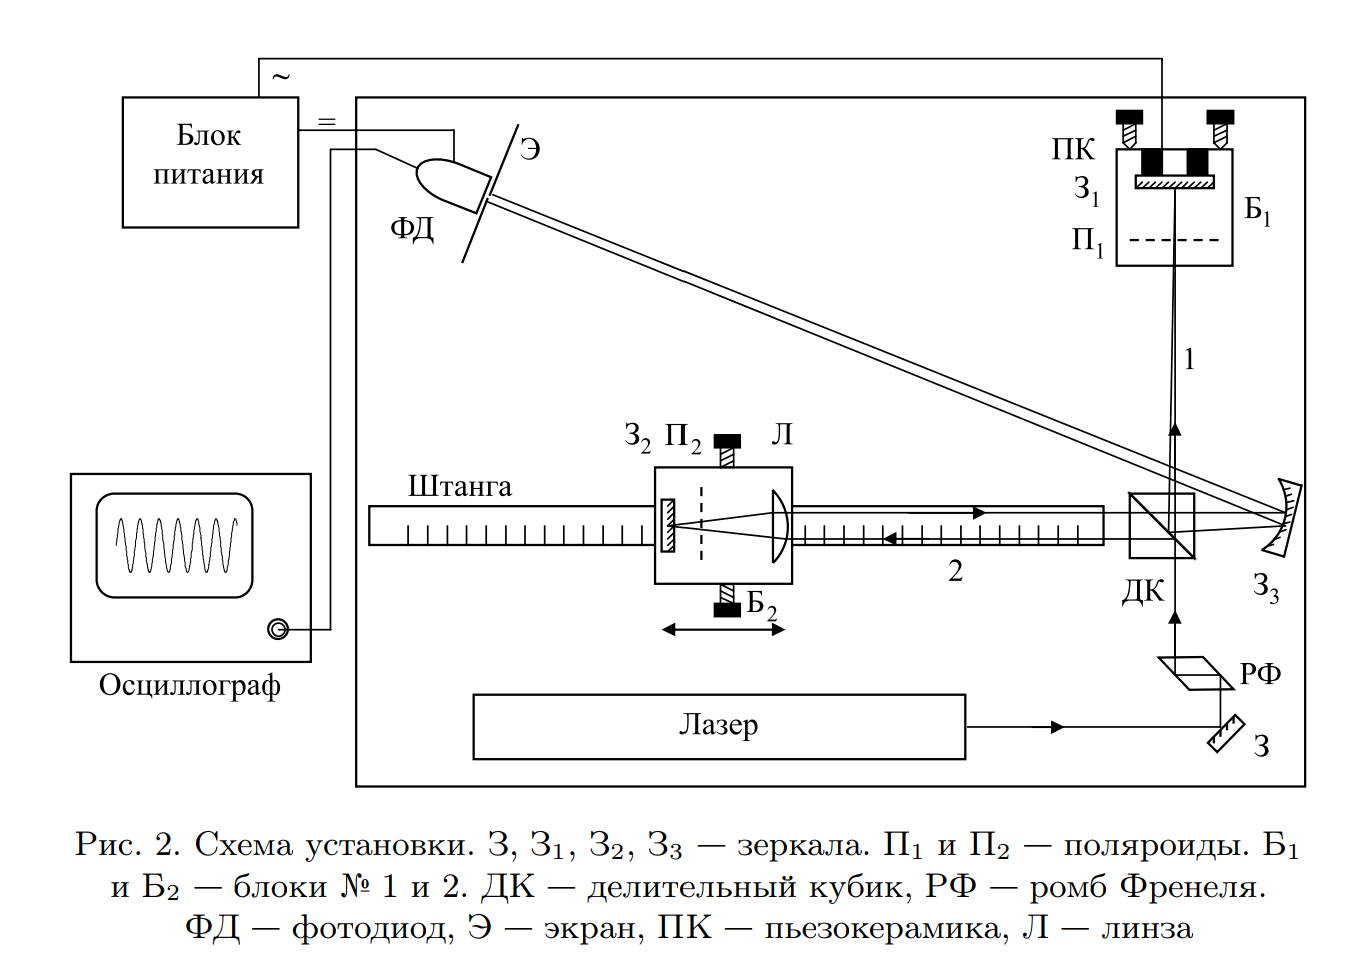
\includegraphics[scale=0.9]{pics/setup.png}
    \end{center}
\end{figure}

В работе используется интерферометр Майкельсона (Рис. 2). Луч лазера,
отражённый от зеркала З и прошедший через ромб Френеля (РФ), делится
делительным кубиком ДК на два луча. Первый проходит блок $\text{Б}_1$ с
поляроидом $\text{П}_1$ и зеркалом $\text{З}_1$, прикленным к пьезокерамике,
которая может совершать малые колебания вдоль луча, с возможностью изменения
угла наклона зеркала. Второй проходит блок $\text{Б}_2$ с линзой Л, поляроидом
$\text{П}_2$ и зеркалом $\text{З}_2$ в фокальной плоскости линзы, чтобы
выходящий луч, в отличие от первого, был параллелен входящему. Оба луча,
проходя ДК, попадают на сферическое зеркало $\text{З}_3$ и интерферируют на
экране. Интенсивность света считывается фотодиодом на осциллограф через щель,
параллельную интерфереционным полосам, в центре экрана. На экране осциллографа
наблюдаются колебания с изменяющимся периодом, так как сдфиг фаз у
интерферирующих лучей пропорционален смещению зеркала $\text{З}_1$.

\begin{wrapfigure}[11]{l}{0.4\textwidth}
    \begin{center}
        \vspace{-30pt}
        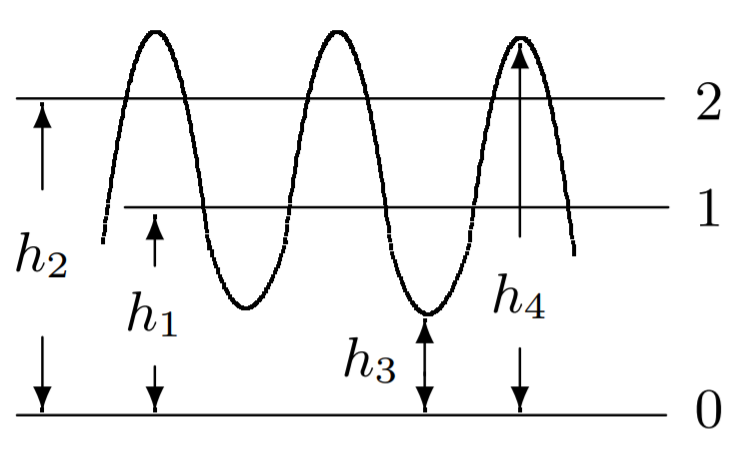
\includegraphics[width = 0.85\linewidth]{pics/osc.png}
    \end{center}
    \caption{Осциллограмма сигналов фотодиода.}
    \label{fig:osc}
\end{wrapfigure}
\vspace{10pt}
По картине на экране осциллографа можно определить параметры видности по следующим формулам:
\begin{equation}
    \delta = \dfrac{h_1}{h_2},
\end{equation}
\begin{equation}
    \V = \dfrac{h_4 - h_3}{h_4 + h_3},
\end{equation}

Здесь 0 -- уровень при отсутствии лучей, 1 и 2 -- при закрытии одного из них.
Используя $\delta$, можно рассчитать $\V_1$ по формуле (5). \vspace{20pt}

При условии одинаковой поляризации лучей ($\alpha = 0$),
\begin{equation}
    \V_2 = \dfrac{\V}{\V_1}.
\end{equation}
Если же разность хода отсутствует ($l = 0$), то
\begin{equation}
    \V_3 = \dfrac{\V}{\V_1}.
\end{equation}

\section{Результаты измерений и обработка результатов}
\subsection{Изучение поляризации лазера}
Вращая поляризатор $\text{П}_1$, мы можем наблюдать изменение видности.

\begin{table}[H]
    \centering
    \caption{Результаты измерений}
    \begin{tabular}{|c|c|c|c|c|c|c|c|c|c|c|c|}
        \hline
        $\beta,~1^\circ$    & 180   & 170   & 160   & 150   & 140   & 130   & 120   & 110   & 100   & 90    & 80    \\ \hline
        $h_1,~\mathrm{div}$ & 3.8   & 3.0   & 2.6   & 2.0   & 2.4   & 2.0   & 1.9   & 1.8   & 1.4   & 1.5   & 1.0   \\ \hline
        $h_2,~\mathrm{div}$ & 2.3   & 2.8   & 2.7   & 3.0   & 2.5   & 2.8   & 2.9   & 3.0   & 3.8   & 4.1   & 5.0   \\ \hline
        $h_3,~\mathrm{div}$ & 8.0   & 8.0   & 8.0   & 8.0   & 8.0   & 8.0   & 8.0   & 8.0   & 8.0   & 8.0   & 8.0   \\ \hline
        $h_4,~\mathrm{div}$ & 4.2   & 3.4   & 2.6   & 2.0   & 1.7   & 1.5   & 1.4   & 1.6   & 2.5   & 3.3   & 4.2   \\ \hline
        $\V$                & 0.311 & 0.404 & 0.509 & 0.600 & 0.649 & 0.684 & 0.702 & 0.667 & 0.524 & 0.416 & 0.311 \\ \hline
        $\delta$            & 1.652 & 1.071 & 0.963 & 0.667 & 0.960 & 0.714 & 0.655 & 0.600 & 0.368 & 0.366 & 0.200 \\ \hline
        $\V_1$              & 0.969 & 0.999 & 1.000 & 0.980 & 1.000 & 0.986 & 0.978 & 0.968 & 0.887 & 0.886 & 0.745 \\ \hline
        $\V_3$              & 0.321 & 0.404 & 0.510 & 0.612 & 0.650 & 0.694 & 0.718 & 0.689 & 0.590 & 0.470 & 0.418 \\ \hline
        $\sigma(\V_3)$      & 0.019 & 0.018 & 0.019 & 0.024 & 0.021 & 0.024 & 0.026 & 0.027 & 0.041 & 0.036 & 0.062 \\ \hline
    \end{tabular}
    \label{tab:results}
\end{table}
Примечание: считается, что погрешность измерений $\sigma(h) = 0.1~\mathrm{div}$, в силу размера деления осциллографа.

\begin{figure}[H]
    \centering
    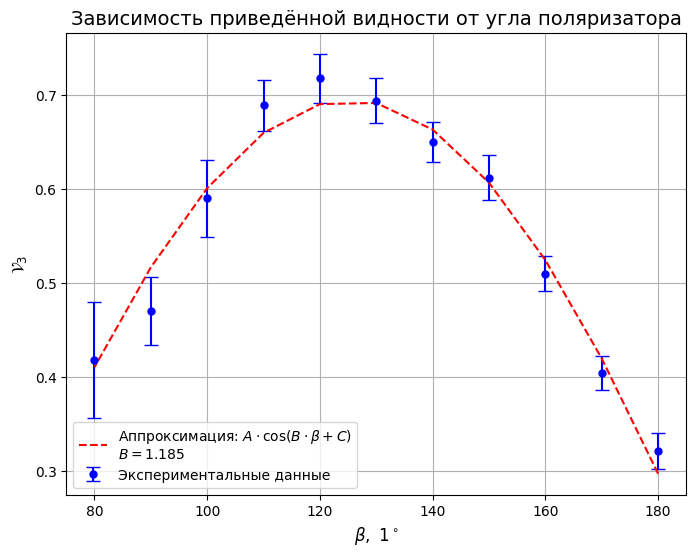
\includegraphics[width = 0.85\linewidth]{pics/2.png}
    \caption{Зависимость приведенной видности от угла поляризатора}
\end{figure}
Как видно, полученная зависимость аппроксимируется косинусом угла. Из чего следует, что лазер излучает линейно поляризованный свет.

\subsection{Изучение зависимости видности от разности хода}
Снимем зависимости $h_1,~h_2,~h_3,~h_4~(l)$. Для удобства чтения данные
перенесены в раздел \ref{addition}, приложение. Отобразим полученную
зависимость на графике.
\begin{figure}[H]
    \centering
    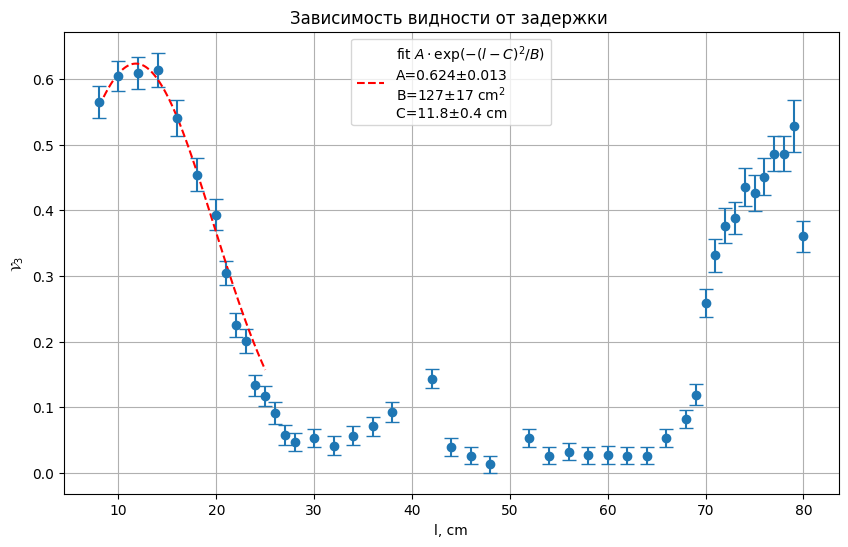
\includegraphics[width = 0.85\linewidth]{pics/V3(L).png}
    \caption{Зависимость видности от разности хода}
\end{figure}

Видно, что не удалось снять ярко выраженный второй максимум, но видно, что
расстояние между максимумами действительно составило $\approx 65~\mathrm{cm}$,
что соответствует расстоянию между зеркалами в лазере. Также медленная
перестройка мод в среднем диапазоне мешала снять последовательные точки, что
видно на графике как некоторые "прыжки" зависимости.

Однако, достаточно хорошо удалось снять первый максимум; приблизим его
гауссианом. Полуширина составит $2\sqrt{B\ln{2}} \approx
    (9.4\pm0.6)~\mathrm{cm}$. В таком случае $$ \Delta F = \dfrac{0.26c}{l_{1/2}}
    \approx (0.83\pm0.06)~\mathrm{GHz}$$ -- полуширина диапазона генерации лазера.

Межмодовое расстояние $\Delta \nu = \dfrac{c}{2L} \approx 0.23\GHz$. Тогда
определим число мод, укладывающиеся в интервал генерации: $$N \approx 1 + 2
    \dfrac{0.83\GHz}{0.23\GHz} \approx 8$$
\section{Обсуждение результатов и выводы}
Было исследовано влияние поляризации и относительной задержки лучей при
интерференции на видность интерференционной картины от света, испущенного
лазером. С помощью полученных зависимостей можно определить тип поляризации
света, генерируемого лазером: после прохождения ромба Френеля свет имел
круговую поляризацию, а значит лазер генерирует линейно поляризованный свет.
Кроме того, была получена правдоподобная картина зависимости видности
интерференционной картины от относительной задержки лучей, с ухудшением
качества данных в середние диапазона. Анализ позволил оценить диапазон
генерации лазера и удостовериться в величине межмодового расстояния, а значит и
получить количество генерируемых мод ($\approx 8$).

\newpage
\section{Приложение}
\label{addition}
\begin{table}[h!]
    \centering
    \caption{Зависимость видности от базы интерферометра (часть 1)}
    \begin{tabular}{|c|c|c|c|c|c|c|c|c|c|c|}
        \hline
        $l,~\mathrm{cm}$    & 8     & 10    & 12    & 14    & 16    & 18    & 20    & 21    & 22    & 23    \\
        \hline
        $h_1,~\mathrm{div}$ & 2.0   & 2.2   & 2.1   & 2.0   & 1.8   & 1.9   & 1.9   & 2.6   & 4.4   & 5.4   \\
        \hline
        $h_2,~\mathrm{div}$ & 3.0   & 2.8   & 3.0   & 3.1   & 3.6   & 3.8   & 4.0   & 3.5   & 2.2   & 2.4   \\
        \hline
        $h_3,~\mathrm{div}$ & 8.0   & 8.0   & 8.0   & 8.0   & 8.0   & 8.0   & 8.0   & 8.0   & 8.0   & 8.0   \\
        \hline
        $h_4,~\mathrm{div}$ & 2.3   & 2.0   & 2.0   & 2.0   & 2.6   & 3.2   & 3.7   & 4.3   & 5.2   & 5.5   \\
        \hline
        $V$                 & 0.553 & 0.600 & 0.600 & 0.600 & 0.509 & 0.429 & 0.368 & 0.301 & 0.212 & 0.185 \\
        \hline
        $\delta$            & 0.667 & 0.786 & 0.700 & 0.645 & 0.500 & 0.500 & 0.475 & 0.743 & 2.000 & 2.250 \\
        \hline
        $V_1$               & 0.980 & 0.993 & 0.984 & 0.976 & 0.943 & 0.943 & 0.935 & 0.989 & 0.943 & 0.923 \\
        \hline
        $V_3$               & 0.565 & 0.604 & 0.610 & 0.614 & 0.540 & 0.455 & 0.393 & 0.304 & 0.225 & 0.201 \\
        \hline
        $\sigma(V_3)$       & 0.019 & 0.020 & 0.020 & 0.020 & 0.019 & 0.018 & 0.017 & 0.016 & 0.015 & 0.015 \\
        \hline
    \end{tabular}
\end{table}

\begin{table}[h!]
    \centering
    \caption{Зависимость видности от базы интерферометра (часть 2)}
    \begin{tabular}{|c|c|c|c|c|c|c|c|c|c|c|}
        \hline
        $l,~\mathrm{cm}$    & 24    & 25    & 26    & 27    & 28    & 30    & 32    & 34    & 36    & 38    \\
        \hline
        $h_1,~\mathrm{div}$ & 4.7   & 4.6   & 5.4   & 5.3   & 4.5   & 4.2   & 5.1   & 5.2   & 5.0   & 4.9   \\
        \hline
        $h_2,~\mathrm{div}$ & 2.5   & 2.4   & 2.0   & 2.3   & 3.1   & 3.3   & 2.6   & 2.5   & 2.5   & 2.6   \\
        \hline
        $h_3,~\mathrm{div}$ & 8.0   & 8.0   & 8.0   & 8.0   & 8.0   & 8.0   & 8.0   & 8.0   & 8.0   & 8.0   \\
        \hline
        $h_4,~\mathrm{div}$ & 6.2   & 6.4   & 6.8   & 7.2   & 7.3   & 7.2   & 7.4   & 7.2   & 7.0   & 6.7   \\
        \hline
        $V$                 & 0.127 & 0.111 & 0.081 & 0.053 & 0.046 & 0.053 & 0.039 & 0.053 & 0.067 & 0.088 \\
        \hline
        $\delta$            & 1.880 & 1.917 & 2.700 & 2.304 & 1.452 & 1.273 & 1.962 & 2.080 & 2.000 & 1.885 \\
        \hline
        $V_1$               & 0.952 & 0.949 & 0.888 & 0.919 & 0.983 & 0.993 & 0.946 & 0.937 & 0.943 & 0.952 \\
        \hline
        $V_3$               & 0.133 & 0.117 & 0.091 & 0.057 & 0.047 & 0.053 & 0.041 & 0.056 & 0.071 & 0.093 \\
        \hline
        $\sigma(V_3)$       & 0.014 & 0.014 & 0.014 & 0.013 & 0.013 & 0.013 & 0.013 & 0.013 & 0.013 & 0.015 \\
        \hline
    \end{tabular}
\end{table}

\begin{table}[h!]
    \centering
    \caption{Зависимость видности от базы интерферометра (часть 3)}
    \begin{tabular}{|c|c|c|c|c|c|c|c|c|c|c|}
        \hline
        $l,~\mathrm{cm}$    & 42    & 44    & 46    & 48    &  & 52    & 54    & 56    & 58    & 60    \\
        \hline
        $h_1,~\mathrm{div}$ & 3.4   & 4.4   & 4.4   & 3.1   &  & 3.5   & 4.0   & 4.0   & 5.0   & 5.2   \\
        \hline
        $h_2,~\mathrm{div}$ & 3.1   & 3.2   & 3.4   & 4.8   &  & 4.2   & 3.8   & 3.7   & 3.1   & 2.6   \\
        \hline
        $h_3,~\mathrm{div}$ & 8.0   & 8.0   & 8.0   & 8.0   &  & 8.0   & 8.0   & 8.0   & 8.0   & 8.0   \\
        \hline
        $h_4,~\mathrm{div}$ & 6.0   & 7.4   & 7.6   & 7.8   &  & 7.2   & 7.6   & 7.5   & 7.6   & 7.6   \\
        \hline
        $V$                 & 0.143 & 0.039 & 0.026 & 0.013 &  & 0.053 & 0.026 & 0.032 & 0.026 & 0.026 \\
        \hline
        $\delta$            & 1.097 & 1.375 & 1.294 & 0.646 &  & 0.833 & 1.053 & 1.081 & 1.613 & 2.000 \\
        \hline
        $V_1$               & 0.999 & 0.987 & 0.992 & 0.977 &  & 0.996 & 1.000 & 0.999 & 0.972 & 0.943 \\
        \hline
        $V_3$               & 0.143 & 0.039 & 0.026 & 0.013 &  & 0.053 & 0.026 & 0.054 & 0.026 & 0.027 \\
        \hline
        $\sigma(V_3)$       & 0.014 & 0.013 & 0.013 & 0.013 &  & 0.013 & 0.001 & 0.013 & 0.013 & 0.013 \\
        \hline
    \end{tabular}
\end{table}

\begin{table}[h!]
    \centering
    \caption{Зависимость видности от базы интерферометра (часть 4)}
    \begin{tabular}{|c|c|c|c|c|c|c|c|c|c|c|}
        \hline
        $l,~\mathrm{cm}$    & 62    & 64    & 66    & 68    & 69    & 70    & 71    & 72    & 73    & 74    \\
        \hline
        $h_1,~\mathrm{div}$ & 4.7   & 4.4   & 4.1   & 3.9   & 5.0   & 4.8   & 4.6   & 4.4   & 4.2   & 4.4   \\
        \hline
        $h_2,~\mathrm{div}$ & 3.2   & 3.4   & 3.7   & 3.3   & 2.4   & 1.8   & 1.6   & 1.6   & 1.8   & 1.5   \\
        \hline
        $h_3,~\mathrm{div}$ & 8.0   & 8.0   & 8.0   & 8.0   & 8.0   & 8.0   & 8.0   & 8.0   & 8.0   & 8.0   \\
        \hline
        $h_4,~\mathrm{div}$ & 7.6   & 7.6   & 7.2   & 6.8   & 6.4   & 5.0   & 4.4   & 4.0   & 3.8   & 3.6   \\
        \hline
        $V$                 & 0.026 & 0.026 & 0.053 & 0.081 & 0.111 & 0.231 & 0.290 & 0.333 & 0.356 & 0.379 \\
        \hline
        $\delta$            & 1.469 & 1.294 & 1.108 & 1.182 & 2.083 & 2.667 & 2.875 & 2.750 & 2.333 & 2.933 \\
        \hline
        $V_1$               & 0.982 & 0.992 & 0.999 & 0.997 & 0.936 & 0.891 & 0.875 & 0.884 & 0.917 & 0.871 \\
        \hline
        $V_3$               & 0.026 & 0.026 & 0.053 & 0.081 & 0.119 & 0.259 & 0.332 & 0.377 & 0.388 & 0.436 \\
        \hline
        $\sigma(V_3)$       & 0.013 & 0.013 & 0.010 & 0.002 & 0.010 & 0.015 & 0.018 & 0.018 & 0.015 & 0.019 \\
        \hline
    \end{tabular}
\end{table}

\begin{table}[h!]
    \centering
    \caption{Зависимость видности от базы интерферометра (часть 5)}
    \begin{tabular}{|c|c|c|c|c|c|c|}
        \hline
        $l,~\mathrm{cm}$    & 75    & 76    & 77    & 78    & 79    & 80    \\
        \hline
        $h_1,~\mathrm{div}$ & 4.3   & 4.2   & 3.8   & 3.8   & 4.2   & 4.0   \\
        \hline
        $h_2,~\mathrm{div}$ & 1.6   & 1.6   & 1.8   & 1.8   & 1.1   & 1.8   \\
        \hline
        $h_3,~\mathrm{div}$ & 8.0   & 8.0   & 8.0   & 8.0   & 8.0   & 8.0   \\
        \hline
        $h_4,~\mathrm{div}$ & 3.6   & 3.4   & 3.0   & 3.0   & 3.2   & 4.0   \\
        \hline
        $V$                 & 0.379 & 0.404 & 0.455 & 0.455 & 0.429 & 0.333 \\
        \hline
        $\delta$            & 2.688 & 2.625 & 2.111 & 2.111 & 3.818 & 2.222 \\
        \hline
        $V_1$               & 0.889 & 0.894 & 0.934 & 0.934 & 0.811 & 0.925 \\
        \hline
        $V_3$               & 0.427 & 0.451 & 0.487 & 0.487 & 0.528 & 0.360 \\
        \hline
        $\sigma(V_3)$       & 0.017 & 0.017 & 0.014 & 0.018 & 0.018 & 0.017 \\
        \hline
    \end{tabular}
\end{table}

\end{document}
